\sectionthree{DFAs are as Powerful as NFAs}
\begin{python0}
  from solutions import *; clear()
\end{python0}

\begin{thm} \mbox{}
 \begin{tightlist}
 \item[(a)] If $M$ is a $\DFA$, then there is an $\NFA$ say $N$ such
  that $L(M) = L(N)$.
 \item[(b)] If $N$ is an $\NFA$, then there is a $\DFA$ say $D$ such
 that $L(N) = L(D)$.
 \end{tightlist}
\end{thm}

I will call this the \lq\lq $\NFA = \DFA$" theorem. (I made this name up
myself, it's not standard).

So although the NFA is more flexible than the definition of a DFA
(so that every DFA is an NFA almost by definition),
it turns out the collection of languages described by DFAs and NFAs
are actually the same -- you can't describe a larger collection of languages.
Here a picture:

\begin{center}
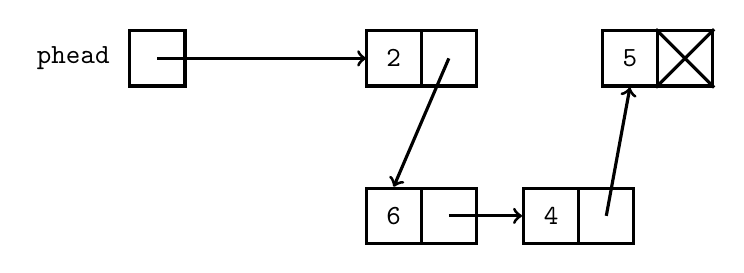
\begin{tikzpicture}

\draw (0.35, 0.35)
  node[draw, line width=0.04cm, , color=black,
       rounded corners=0cm, inner sep=0cm] {

\begin{minipage}[t][0.7cm]{0.7cm}
\mbox{}

\end{minipage}

};\draw (0.35, 0.35) node[color=black] {{\texttt{2}}};
\draw (1.0499999999999998, 0.35)
  node[draw, line width=0.04cm, , color=black,
       rounded corners=0cm, inner sep=0cm] {

\begin{minipage}[t][0.7cm]{0.7cm}
\mbox{}

\end{minipage}

};\draw (1.0499999999999998, 0.35) node[color=black] {{\texttt{}}};
\draw (0.35, -1.65)
  node[draw, line width=0.04cm, , color=black,
       rounded corners=0cm, inner sep=0cm] {

\begin{minipage}[t][0.7cm]{0.7cm}
\mbox{}

\end{minipage}

};\draw (0.35, -1.65) node[color=black] {{\texttt{6}}};
\draw (1.0499999999999998, -1.65)
  node[draw, line width=0.04cm, , color=black,
       rounded corners=0cm, inner sep=0cm] {

\begin{minipage}[t][0.7cm]{0.7cm}
\mbox{}

\end{minipage}

};\draw (1.0499999999999998, -1.65) node[color=black] {{\texttt{}}};
\draw (2.35, -1.65)
  node[draw, line width=0.04cm, , color=black,
       rounded corners=0cm, inner sep=0cm] {

\begin{minipage}[t][0.7cm]{0.7cm}
\mbox{}

\end{minipage}

};\draw (2.35, -1.65) node[color=black] {{\texttt{4}}};
\draw (3.0500000000000003, -1.65)
  node[draw, line width=0.04cm, , color=black,
       rounded corners=0cm, inner sep=0cm] {

\begin{minipage}[t][0.7cm]{0.7cm}
\mbox{}

\end{minipage}

};\draw (3.0500000000000003, -1.65) node[color=black] {{\texttt{}}};
\draw (3.35, 0.35)
  node[draw, line width=0.04cm, , color=black,
       rounded corners=0cm, inner sep=0cm] {

\begin{minipage}[t][0.7cm]{0.7cm}
\mbox{}

\end{minipage}

};\draw (3.35, 0.35) node[color=black] {{\texttt{5}}};
\draw (4.05, 0.35)
  node[draw, line width=0.04cm, , color=black,
       rounded corners=0cm, inner sep=0cm] {

\begin{minipage}[t][0.7cm]{0.7cm}
\mbox{}

\end{minipage}

};\draw (4.05, 0.35) node[color=black] {{\texttt{}}};\draw[line width=0.04cm,black,->] (1.05,0.35) to  (0.35,-1.28);
\draw[line width=0.04cm,black,->] (1.05,-1.65) to  (1.98,-1.65);
\draw[line width=0.04cm,black,->] (3.05,-1.65) to  (3.35,-0.02);
\draw[line width=0.04cm,black] (3.68,0.72) to  (4.42,-0.02);
\draw[line width=0.04cm,black] (4.42,0.72) to  (3.68,-0.02);

\draw (-2.65, 0.35)
  node[draw, line width=0.04cm, , color=black,
       rounded corners=0cm, inner sep=0cm] {

\begin{minipage}[t][0.7cm]{0.7cm}
\mbox{}

\end{minipage}

};\draw (-2.65, 0.35) node[color=black] {{\texttt{}}};\draw[line width=0.04cm,black,->] (-2.65,0.35) to  (0,0.35);

\draw (-3.7199999999999998, 0.35)
  node[draw, line width=0.04cm, , color=white,
       rounded corners=0cm, inner sep=0cm] {

\begin{minipage}[t][0.1cm]{0.1cm}
\mbox{}

\end{minipage}

};\draw (-3.7199999999999998, 0.35) node[color=black] {{\texttt{phead}}};
\end{tikzpicture}

\end{center}



Recall that a language is regular if it's the language
accepted by a DFA.
So $\Reg_\Sigma$ is the set of hits of $\DFA_\Sigma$ in the above diagram.
The set of machines, $\NFA_\Sigma$, hits
the same set of languages as $\Reg_\Sigma$ -- you don't get more.

The proof of part (a) of the $\NFA=\DFA$ is easy and I'll leave it as an
exercise. Make sure you do it on your own.

Now to prove part (b) of $\NFA=\DFA$. Believe it or not, the proof is
easy too. Furthermore, the prove is constructive. The point is to
look very carefully at the definitions above especially of the
computation and to massage the objects in the definition.

Let $N = (\Sigma,Q,q_0,F,\delta)$ be an $\NFA$. 
Don't forget that the transition function $\delta$ has the following form:
\[
\delta: Q \times \Sigma_\ep \rightarrow P(Q)
\] 
where $\Sigma_\ep = \Sigma \cup \{\epsilon\}$ and $P(Q)$ is the 
powerset of $Q$.
Furthermore, I'm extending the $\delta$ to accept $(S, x)$
where $S$ is a \textit{set} of states.
This is done in the following (obvious!) way:
\[
\delta(S, c) = \bigcup_{q \in S} \delta(q, c)
\]
where $S \subset Q$ and $c \in \Sigma_\ep$.

Suppose it's possible
to construct a $\DFA$ 
\[
M = (\Sigma,Q^{\DFA}, q_0^{\DFA}, F^{\DFA}, \delta^{\DFA})
\]
so that $L(M) = L(N)$. What would $M$ look like?

Take a look at the definition of computation:
\[
 (S,cx) \vdash (\overline{\delta(S,c)}, x)
\]
where $S \subseteq Q$ and $c \in \Sigma_\ep$.
Now look that definition of the computation of a $\DFA$
that we would like to have:
\[
 (q,cx) \vdash (\delta^{\DFA}(q,c),x)
\]

Doesn't that tell you that the DFA should somehow have
\textbf{sets}
as states?!?! In particular, the sets are
\textbf{subsets} of
$Q$. See it? Just to repeat, $Q^{\DFA}$ is a set of set of states.
Therefore $Q^{\DFA} \subseteq P(Q)$. Maybe we need $Q^{\DFA} =
P(Q)$??? We'll see.

What about $\delta^{\DFA}$ for our guess? When you compare the above
computations symbolically, doesn't that say that for if $S \in
Q^{\DFA}$ and $a\in \Sigma$, then
\[
 \delta^{\DFA}(S,c) 
\defeq \overline{\delta(S,c)}
= \overline{\bigcup_{q \in S} \delta(q,c)}
\]
In that case,
\[
 (S,ax) \vdash (\overline{\delta(S,c)}, x)
\]
does become:
\[
 (S,ax) \vdash (\delta^{\DFA}(S,c), x)
\]
Viola!!!

So far we have $Q^{\DFA}$ and $\delta^{\DFA}$. Think about it. We
start our machine with $q_0$. But our $Q^{\DFA}$ is a set of set of
states. So the initial state is not $q_0$ but $\overline{\{q_0\}}$. 
Therefore
we define the initial state of our DFA as $q_0^{\DFA} \defeq
\overline{\{q_0\}}$. 
And of course $q_0^{\DFA} \in Q^{\DFA}$, at least if we let
$Q^{\DFA} = P(Q)$.

What about the accepting states $F^{\DFA}$? You already know that a
string is accepted by the NFA if you have at least one computation
leading to one accepting state. Formally our above definition says
that $x$ is accepted if
\[
 (\overline{\{q_0\}}, x) \vdash^* (S, \ep), \quad S \cap F \neq \emptyset
\]
Well $\ldots$ obviously we define $F^{\DFA}$ to be those sets of
state that contain at least one accepting state in $F$ of the NFA:
\[
 F^{\DFA} \defeq \{S \in Q^{\DFA} \,|\, S \cap F \neq \emptyset \}
\]
I mean, what else can it be?!?

As an example of a specific state of our new $\DFA$,
note that since the states of the new $\DFA$ are the
subset of $Q$ (the states of the $\NFA$)
and the emptyset
$\emptyset$ is an element of $P(Q)$,
our $\DFA$ has a state labeled as $\{\}$.
Note that by our definition above
\[
\delta^{\DFA}(\emptyset, c)
= \emptyset
\]
(Right?)

So let's begin the formal proof of $\NFA=\DFA$ part (b).

\begin{proof}
Let $N = (\Sigma, Q, q_0, F, \delta)$ be an $\NFA$. 
Given a subset $S$ of $Q$, $\overline{S}$ denotes the $\epsilon$-closure
of $S$.
Define $M =
(\Sigma$, $Q^{\DFA}$, $q_0^{\DFA}$, $F^{\DFA}$, $\delta^{\DFA})$ as
follows: 
 \begin{itemize}
 \item $Q^{\DFA} = P(Q)$
 \item $q_0^{\DFA} = \overline{\{q_0\}}$
 \item $F^{\DFA} = \{ S \in Q^{\DFA} \,|\, S \cap F \neq \emptyset \}$
 \item $\delta^{\DFA} : Q \times \Sigma \rightarrow Q$ is defined as
 follows: Let $S \in Q^{\DFA}$ and $c \in \Sigma$. Then
 \[
   \delta^{\DFA}(S,c) = \overline{\bigcup_{q \in S} \delta(q,c)}
 \]
 \end{itemize}
Then 
\[
L(M) = L(N)
\]
(Details are left to the reader.)
\end{proof}

The above NFA-to-DFA construction is sometimes called the
\defone{subset construction} or the
\tinysidebarskip\defone{powerset construction}\sidebarskip{0pt}.


I hope you recall that $|P(Q)| = 2^{|Q|}$. 
That means that the
resulting DFA is big when compared against the original NFA. 
Here size is measured in terms of the
number of states. We'll see later that there is an algorithm to
simplify DFAs.

Of course if there is a state that cannot be reached from the initial
node, you can just remove it. 
So we usually don't draw \textit{all} the subsets of $Q$ (of the $\NFA$)
for the $\DFA$. 
We usually start with the start state of the $\DFA$ 
(i.e., the $\ep$--closure of the start state of the $\NFA$)
and keep adding $\DFA$ states until the $\DFA$ is completed.
So in your $\NFA$ has 5 states.
The complete subset construction gives you a $\DFA$ with $2^5 = 32$ states.
However if you only include states reachable for the start state
of the $\DFA$, the $\DFA$ might be smaller;
the other states cannot be reached the start state of the $\DFA$
and hence does not take part in the computation of a string.
(They can be included of course.)

%-*-latex-*-

\begin{ex} 
  \label{ex:prob-00}
  \tinysidebar{\debug{exercises/{disc-prob-28/question.tex}}}

  \solutionlink{sol:prob-00}
  \qed
\end{ex} 
\begin{python0}
from solutions import *
add(label="ex:prob-00",
    srcfilename='exercises/discrete-probability/prob-00/answer.tex') 
\end{python0}


Note that the above DFA does accept the same language as the 
NFA we started with, i.e., $\{\}$.

Note that the subset construction does not
necessarily give the simplest DFA.
Clearly the simplest DFA that accepts $\{\}$ is
\begin{center}
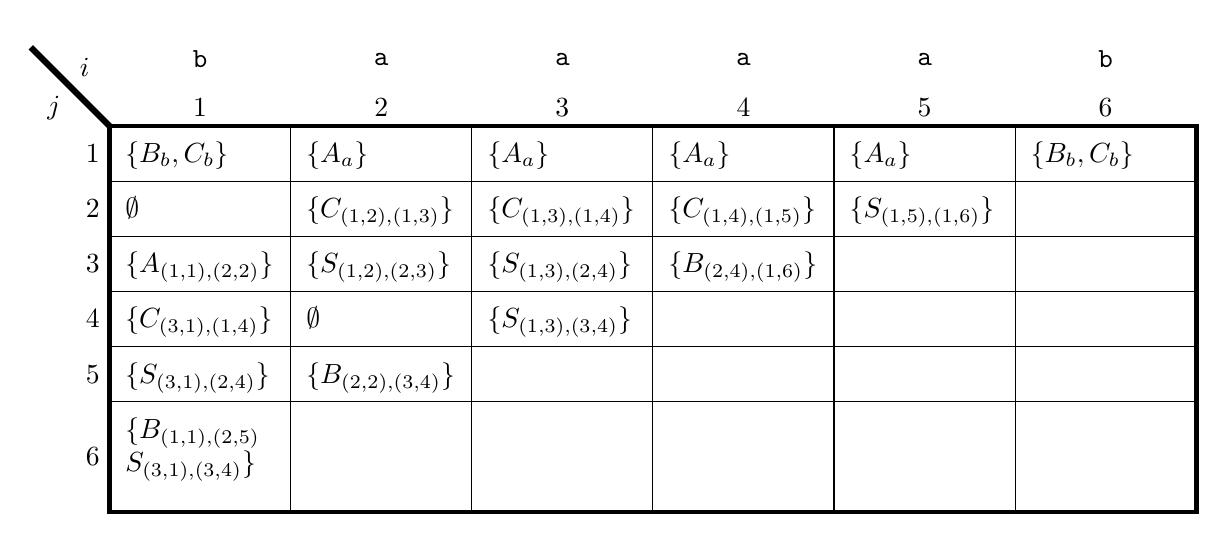
\begin{tikzpicture}

\draw (1.15, -0.35)
  node[draw, , , color=black,
       rounded corners=0cm, inner sep=0.2cm] {

\begin{minipage}[t][0.3cm]{1.9cm}
\mbox{}

\end{minipage}

};
\draw (1.15, -0.35) node[color=black,
 inner sep=0.2cm] {
 
\begin{minipage}[t][0.3cm]{1.9cm}
$\{B_b,C_b\}$
\end{minipage}

};
\draw (3.4499999999999997, -0.35)
  node[draw, , , color=black,
       rounded corners=0cm, inner sep=0.2cm] {

\begin{minipage}[t][0.3cm]{1.9cm}
\mbox{}

\end{minipage}

};
\draw (3.4499999999999997, -0.35) node[color=black,
 inner sep=0.2cm] {
 
\begin{minipage}[t][0.3cm]{1.9cm}
$\{A_a\}$
\end{minipage}

};
\draw (5.75, -0.35)
  node[draw, , , color=black,
       rounded corners=0cm, inner sep=0.2cm] {

\begin{minipage}[t][0.3cm]{1.9cm}
\mbox{}

\end{minipage}

};
\draw (5.75, -0.35) node[color=black,
 inner sep=0.2cm] {
 
\begin{minipage}[t][0.3cm]{1.9cm}
$\{A_a\}$
\end{minipage}

};
\draw (8.049999999999999, -0.35)
  node[draw, , , color=black,
       rounded corners=0cm, inner sep=0.2cm] {

\begin{minipage}[t][0.3cm]{1.9cm}
\mbox{}

\end{minipage}

};
\draw (8.049999999999999, -0.35) node[color=black,
 inner sep=0.2cm] {
 
\begin{minipage}[t][0.3cm]{1.9cm}
$\{A_a\}$
\end{minipage}

};
\draw (10.35, -0.35)
  node[draw, , , color=black,
       rounded corners=0cm, inner sep=0.2cm] {

\begin{minipage}[t][0.3cm]{1.9cm}
\mbox{}

\end{minipage}

};
\draw (10.35, -0.35) node[color=black,
 inner sep=0.2cm] {
 
\begin{minipage}[t][0.3cm]{1.9cm}
$\{A_a\}$
\end{minipage}

};
\draw (12.65, -0.35)
  node[draw, , , color=black,
       rounded corners=0cm, inner sep=0.2cm] {

\begin{minipage}[t][0.3cm]{1.9cm}
\mbox{}

\end{minipage}

};
\draw (12.65, -0.35) node[color=black,
 inner sep=0.2cm] {
 
\begin{minipage}[t][0.3cm]{1.9cm}
$\{B_b,C_b\}$
\end{minipage}

};
\draw (1.15, -1.0499999999999998)
  node[draw, , , color=black,
       rounded corners=0cm, inner sep=0.2cm] {

\begin{minipage}[t][0.3cm]{1.9cm}
\mbox{}

\end{minipage}

};
\draw (1.15, -1.0499999999999998) node[color=black,
 inner sep=0.2cm] {
 
\begin{minipage}[t][0.3cm]{1.9cm}
$\emptyset$
\end{minipage}

};
\draw (3.4499999999999997, -1.0499999999999998)
  node[draw, , , color=black,
       rounded corners=0cm, inner sep=0.2cm] {

\begin{minipage}[t][0.3cm]{1.9cm}
\mbox{}

\end{minipage}

};
\draw (3.4499999999999997, -1.0499999999999998) node[color=black,
 inner sep=0.2cm] {
 
\begin{minipage}[t][0.3cm]{1.9cm}
$\{C_{(1,2),(1,3)}\}$
\end{minipage}

};
\draw (5.75, -1.0499999999999998)
  node[draw, , , color=black,
       rounded corners=0cm, inner sep=0.2cm] {

\begin{minipage}[t][0.3cm]{1.9cm}
\mbox{}

\end{minipage}

};
\draw (5.75, -1.0499999999999998) node[color=black,
 inner sep=0.2cm] {
 
\begin{minipage}[t][0.3cm]{1.9cm}
$\{C_{(1,3),(1,4)}\}$
\end{minipage}

};
\draw (8.049999999999999, -1.0499999999999998)
  node[draw, , , color=black,
       rounded corners=0cm, inner sep=0.2cm] {

\begin{minipage}[t][0.3cm]{1.9cm}
\mbox{}

\end{minipage}

};
\draw (8.049999999999999, -1.0499999999999998) node[color=black,
 inner sep=0.2cm] {
 
\begin{minipage}[t][0.3cm]{1.9cm}
$\{C_{(1,4),(1,5)}\}$
\end{minipage}

};
\draw (10.35, -1.0499999999999998)
  node[draw, , , color=black,
       rounded corners=0cm, inner sep=0.2cm] {

\begin{minipage}[t][0.3cm]{1.9cm}
\mbox{}

\end{minipage}

};
\draw (10.35, -1.0499999999999998) node[color=black,
 inner sep=0.2cm] {
 
\begin{minipage}[t][0.3cm]{1.9cm}
$\{S_{(1,5),(1,6)}\}$
\end{minipage}

};
\draw (12.65, -1.0499999999999998)
  node[draw, , , color=black,
       rounded corners=0cm, inner sep=0.2cm] {

\begin{minipage}[t][0.3cm]{1.9cm}
\mbox{}

\end{minipage}

};
\draw (1.15, -1.7499999999999996)
  node[draw, , , color=black,
       rounded corners=0cm, inner sep=0.2cm] {

\begin{minipage}[t][0.3cm]{1.9cm}
\mbox{}

\end{minipage}

};
\draw (1.15, -1.7499999999999996) node[color=black,
 inner sep=0.2cm] {
 
\begin{minipage}[t][0.3cm]{1.9cm}
$\{A_{(1,1),(2,2)}\}$
\end{minipage}

};
\draw (3.4499999999999997, -1.7499999999999996)
  node[draw, , , color=black,
       rounded corners=0cm, inner sep=0.2cm] {

\begin{minipage}[t][0.3cm]{1.9cm}
\mbox{}

\end{minipage}

};
\draw (3.4499999999999997, -1.7499999999999996) node[color=black,
 inner sep=0.2cm] {
 
\begin{minipage}[t][0.3cm]{1.9cm}
$\{S_{(1,2),(2,3)}\}$
\end{minipage}

};
\draw (5.75, -1.7499999999999996)
  node[draw, , , color=black,
       rounded corners=0cm, inner sep=0.2cm] {

\begin{minipage}[t][0.3cm]{1.9cm}
\mbox{}

\end{minipage}

};
\draw (5.75, -1.7499999999999996) node[color=black,
 inner sep=0.2cm] {
 
\begin{minipage}[t][0.3cm]{1.9cm}
$\{S_{(1,3),(2,4)}\}$
\end{minipage}

};
\draw (8.049999999999999, -1.7499999999999996)
  node[draw, , , color=black,
       rounded corners=0cm, inner sep=0.2cm] {

\begin{minipage}[t][0.3cm]{1.9cm}
\mbox{}

\end{minipage}

};
\draw (8.049999999999999, -1.7499999999999996) node[color=black,
 inner sep=0.2cm] {
 
\begin{minipage}[t][0.3cm]{1.9cm}
$\{B_{(2,4),(1,6)}\}$
\end{minipage}

};
\draw (10.35, -1.7499999999999996)
  node[draw, , , color=black,
       rounded corners=0cm, inner sep=0.2cm] {

\begin{minipage}[t][0.3cm]{1.9cm}
\mbox{}

\end{minipage}

};
\draw (12.65, -1.7499999999999996)
  node[draw, , , color=black,
       rounded corners=0cm, inner sep=0.2cm] {

\begin{minipage}[t][0.3cm]{1.9cm}
\mbox{}

\end{minipage}

};
\draw (1.15, -2.4499999999999997)
  node[draw, , , color=black,
       rounded corners=0cm, inner sep=0.2cm] {

\begin{minipage}[t][0.3cm]{1.9cm}
\mbox{}

\end{minipage}

};
\draw (1.15, -2.4499999999999997) node[color=black,
 inner sep=0.2cm] {
 
\begin{minipage}[t][0.3cm]{1.9cm}
$\{C_{(3,1),(1,4)}\}$
\end{minipage}

};
\draw (3.4499999999999997, -2.4499999999999997)
  node[draw, , , color=black,
       rounded corners=0cm, inner sep=0.2cm] {

\begin{minipage}[t][0.3cm]{1.9cm}
\mbox{}

\end{minipage}

};
\draw (3.4499999999999997, -2.4499999999999997) node[color=black,
 inner sep=0.2cm] {
 
\begin{minipage}[t][0.3cm]{1.9cm}
$\emptyset$
\end{minipage}

};
\draw (5.75, -2.4499999999999997)
  node[draw, , , color=black,
       rounded corners=0cm, inner sep=0.2cm] {

\begin{minipage}[t][0.3cm]{1.9cm}
\mbox{}

\end{minipage}

};
\draw (5.75, -2.4499999999999997) node[color=black,
 inner sep=0.2cm] {
 
\begin{minipage}[t][0.3cm]{1.9cm}
$\{S_{(1,3),(3,4)}\}$
\end{minipage}

};
\draw (8.049999999999999, -2.4499999999999997)
  node[draw, , , color=black,
       rounded corners=0cm, inner sep=0.2cm] {

\begin{minipage}[t][0.3cm]{1.9cm}
\mbox{}

\end{minipage}

};
\draw (10.35, -2.4499999999999997)
  node[draw, , , color=black,
       rounded corners=0cm, inner sep=0.2cm] {

\begin{minipage}[t][0.3cm]{1.9cm}
\mbox{}

\end{minipage}

};
\draw (12.65, -2.4499999999999997)
  node[draw, , , color=black,
       rounded corners=0cm, inner sep=0.2cm] {

\begin{minipage}[t][0.3cm]{1.9cm}
\mbox{}

\end{minipage}

};
\draw (1.15, -3.15)
  node[draw, , , color=black,
       rounded corners=0cm, inner sep=0.2cm] {

\begin{minipage}[t][0.3cm]{1.9cm}
\mbox{}

\end{minipage}

};
\draw (1.15, -3.15) node[color=black,
 inner sep=0.2cm] {
 
\begin{minipage}[t][0.3cm]{1.9cm}
$\{S_{(3,1),(2,4)}\}$
\end{minipage}

};
\draw (3.4499999999999997, -3.15)
  node[draw, , , color=black,
       rounded corners=0cm, inner sep=0.2cm] {

\begin{minipage}[t][0.3cm]{1.9cm}
\mbox{}

\end{minipage}

};
\draw (3.4499999999999997, -3.15) node[color=black,
 inner sep=0.2cm] {
 
\begin{minipage}[t][0.3cm]{1.9cm}
$\{B_{(2,2),(3,4)}\}$
\end{minipage}

};
\draw (5.75, -3.15)
  node[draw, , , color=black,
       rounded corners=0cm, inner sep=0.2cm] {

\begin{minipage}[t][0.3cm]{1.9cm}
\mbox{}

\end{minipage}

};
\draw (8.049999999999999, -3.15)
  node[draw, , , color=black,
       rounded corners=0cm, inner sep=0.2cm] {

\begin{minipage}[t][0.3cm]{1.9cm}
\mbox{}

\end{minipage}

};
\draw (10.35, -3.15)
  node[draw, , , color=black,
       rounded corners=0cm, inner sep=0.2cm] {

\begin{minipage}[t][0.3cm]{1.9cm}
\mbox{}

\end{minipage}

};
\draw (12.65, -3.15)
  node[draw, , , color=black,
       rounded corners=0cm, inner sep=0.2cm] {

\begin{minipage}[t][0.3cm]{1.9cm}
\mbox{}

\end{minipage}

};
\draw (1.15, -4.2)
  node[draw, , , color=black,
       rounded corners=0cm, inner sep=0.2cm] {

\begin{minipage}[t][1.0cm]{1.9cm}
\mbox{}

\end{minipage}

};
\draw (1.15, -4.2) node[color=black,
 inner sep=0.2cm] {
 
\begin{minipage}[t][1.0cm]{1.9cm}
$\{B_{(1,1),(2,5)}$ $S_{(3,1),(3,4)}\}$
\end{minipage}

};
\draw (3.4499999999999997, -4.2)
  node[draw, , , color=black,
       rounded corners=0cm, inner sep=0.2cm] {

\begin{minipage}[t][1.0cm]{1.9cm}
\mbox{}

\end{minipage}

};
\draw (5.75, -4.2)
  node[draw, , , color=black,
       rounded corners=0cm, inner sep=0.2cm] {

\begin{minipage}[t][1.0cm]{1.9cm}
\mbox{}

\end{minipage}

};
\draw (8.049999999999999, -4.2)
  node[draw, , , color=black,
       rounded corners=0cm, inner sep=0.2cm] {

\begin{minipage}[t][1.0cm]{1.9cm}
\mbox{}

\end{minipage}

};
\draw (10.35, -4.2)
  node[draw, , , color=black,
       rounded corners=0cm, inner sep=0.2cm] {

\begin{minipage}[t][1.0cm]{1.9cm}
\mbox{}

\end{minipage}

};
\draw (12.65, -4.2)
  node[draw, , , color=black,
       rounded corners=0cm, inner sep=0.2cm] {

\begin{minipage}[t][1.0cm]{1.9cm}
\mbox{}

\end{minipage}

};\node[anchor=south] at (1.15,0.0) {1};\node[anchor=south] at (3.4499999999999997,0.0) {2};\node[anchor=south] at (5.75,0.0) {3};\node[anchor=south] at (8.049999999999999,0.0) {4};\node[anchor=south] at (10.35,0.0) {5};\node[anchor=south] at (12.65,0.0) {6};\node[anchor=east] at (0,-0.35) {1};\node[anchor=east] at (0,-1.0499999999999998) {2};\node[anchor=east] at (0,-1.7499999999999996) {3};\node[anchor=east] at (0,-2.4499999999999997) {4};\node[anchor=east] at (0,-3.15) {5};\node[anchor=east] at (0,-4.2) {6};
\draw (6.9, -2.45)
  node[draw, line width=0.06cm, , color=black,
       rounded corners=0cm, inner sep=0cm] {

\begin{minipage}[t][4.9cm]{13.8cm}
\mbox{}

\end{minipage}

};\draw[line width=0.08cm,black] (0,0.0) to  (-1,1.0);
\node[anchor=north east] at (-0.5,0.5) {$j$};\node[anchor=south west] at (-0.5,0.5) {$i$};
\draw (1.15, 0.85)
  node[draw, line width=0.1cm, , color=white,
       rounded corners=0cm, inner sep=0cm] {

\begin{minipage}[t][0.7cm]{2.3cm}
\mbox{}

\end{minipage}

};\draw (1.15, 0.85) node[color=black] {{\texttt{b}}};
\draw (3.4499999999999997, 0.85)
  node[draw, line width=0.1cm, , color=white,
       rounded corners=0cm, inner sep=0cm] {

\begin{minipage}[t][0.7cm]{2.3cm}
\mbox{}

\end{minipage}

};\draw (3.4499999999999997, 0.85) node[color=black] {{\texttt{a}}};
\draw (5.75, 0.85)
  node[draw, line width=0.1cm, , color=white,
       rounded corners=0cm, inner sep=0cm] {

\begin{minipage}[t][0.7cm]{2.3cm}
\mbox{}

\end{minipage}

};\draw (5.75, 0.85) node[color=black] {{\texttt{a}}};
\draw (8.05, 0.85)
  node[draw, line width=0.1cm, , color=white,
       rounded corners=0cm, inner sep=0cm] {

\begin{minipage}[t][0.7cm]{2.3cm}
\mbox{}

\end{minipage}

};\draw (8.05, 0.85) node[color=black] {{\texttt{a}}};
\draw (10.35, 0.85)
  node[draw, line width=0.1cm, , color=white,
       rounded corners=0cm, inner sep=0cm] {

\begin{minipage}[t][0.7cm]{2.3cm}
\mbox{}

\end{minipage}

};\draw (10.35, 0.85) node[color=black] {{\texttt{a}}};
\draw (12.65, 0.85)
  node[draw, line width=0.1cm, , color=white,
       rounded corners=0cm, inner sep=0cm] {

\begin{minipage}[t][0.7cm]{2.3cm}
\mbox{}

\end{minipage}

};\draw (12.65, 0.85) node[color=black] {{\texttt{b}}};
\end{tikzpicture}

\end{center}


\lq\lq Simplest" meaning \lq\lq fewest states".

%-*-latex-*-

\begin{ex} 
  \label{ex:prob-00}
  \tinysidebar{\debug{exercises/{disc-prob-28/question.tex}}}

  \solutionlink{sol:prob-00}
  \qed
\end{ex} 
\begin{python0}
from solutions import *
add(label="ex:prob-00",
    srcfilename='exercises/discrete-probability/prob-00/answer.tex') 
\end{python0}

\vspace{3in}

%-*-latex-*-

\begin{ex} 
  \label{ex:prob-00}
  \tinysidebar{\debug{exercises/{disc-prob-28/question.tex}}}

  \solutionlink{sol:prob-00}
  \qed
\end{ex} 
\begin{python0}
from solutions import *
add(label="ex:prob-00",
    srcfilename='exercises/discrete-probability/prob-00/answer.tex') 
\end{python0}


%-*-latex-*-

\begin{ex} 
  \label{ex:prob-00}
  \tinysidebar{\debug{exercises/{disc-prob-28/question.tex}}}

  \solutionlink{sol:prob-00}
  \qed
\end{ex} 
\begin{python0}
from solutions import *
add(label="ex:prob-00",
    srcfilename='exercises/discrete-probability/prob-00/answer.tex') 
\end{python0}


%-*-latex-*-

\begin{ex} 
  \label{ex:prob-00}
  \tinysidebar{\debug{exercises/{disc-prob-28/question.tex}}}

  \solutionlink{sol:prob-00}
  \qed
\end{ex} 
\begin{python0}
from solutions import *
add(label="ex:prob-00",
    srcfilename='exercises/discrete-probability/prob-00/answer.tex') 
\end{python0}

